%----------------------------------------------------------------------------
\chapter{Monitor generálás terv}
%----------------------------------------------------------------------------

\begin{figure}[!ht]
    \centering
    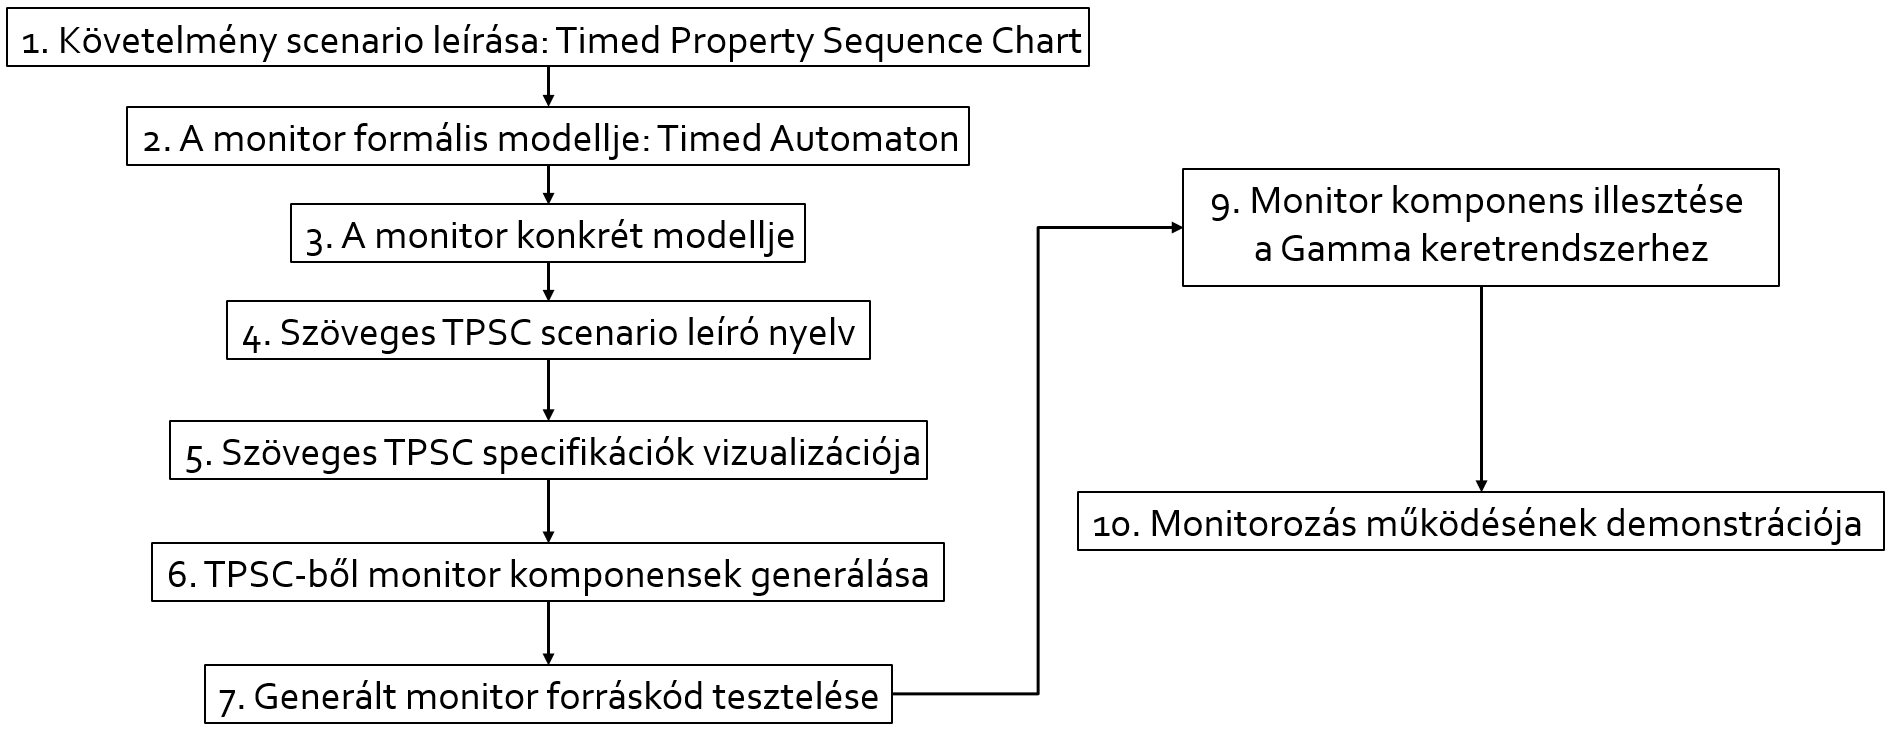
\includegraphics[width=150mm, keepaspectratio]{figures/generation_plan.png}
    \caption{Monitor generátor kibővítése.}
\end{figure}

A cél az, hogy a „Monitor komponensek generálása kontextusfüggő viselkedés ellenőrzése” című szakdolgozatom során elkészített monitor komponens generátort kibővíteni úgy, hogy támogassa időzítési feltételek megadását. A monitor generálás terve látható a 10. ábrán. Először az a feladatunk, hogy a szakdolgozat során definiált szöveges PSC diagram leíró nyelvet kibővitsük a TPSC elemeivel. Ezután az automata generátort kell úgy kibővíteni, hogy a TPSC diagramokból tudjon TA automatákat generálni. Egy monitor forráskód generátor pedig az automata alapján elkészítheti a monitor forráskódját. A Diplomatervezés 1 tárgy keretében a tervnek a negyedik, hatodik és hetedik részeivel foglalkoztam.